\section{Experiments}
\label{sec:diffusion_experiments}

Or main goal in this investigation into diffusion models was to get a better understanding of their performance on a wide range of tasks. We keep in mind the original task of improving an existing motion sequence, but are aware of the other potentials of the model and so do not limit ourselves in scope.


%%%%%%%%%%%%%%%%%%%%%%%%%%%%%%%%%%%%%%%%%%%%%%%%%%%%%%%%%%%%%%%%%%%%%%%%%
% General test cases
%%%%%%%%%%%%%%%%%%%%%%%%%%%%%%%%%%%%%%%%%%%%%%%%%%%%%%%%%%%%%%%%%%%%%%%%%
\subsection{Test Cases}
We present here a variety of different test cases that on which the models performance can be evaluated. The general structure of the evaluation is to generate a sufficiently large number of sequences for each given task, then to import them into blender and visually inspect their quality and how well they acheive each task. We have decided to take a qualitative approach as we are attempting to get a better understanding of the models capabilities, and so this was the path of least resistance to obtain such an understanding in the time that was left after the HuMoR investigation. We note that in the future, if a given task is deemed worth investigation further, or if a significantly larger number of models are being test, more rigorous evaluation metrics would be greatly benefitial.

\subsubsection{Sequence Generation}
To ensure that the model has learned a sensible variety of human motion, we generate a number of sequences from gaussian noise, and check that they contain sufficient diversity, considering that a main indicator of an overfit diffusion model is that of a lack of diversity.

\subsubsection{Denoising}
\TODO{Come up with a better test for this}

\subsubsection{Occluded Legs}
An important situation in which the current Disney Research|Studious model does not perform optimally is that of occluded sequences. To test the ability of the diffusion models to handle this situation, we evaluate the models capabilities to generate the leg motion of an entire motion sequence. We acheive this using the inpainting framework described in \secref{sec:diffusion_method_inpainting}, keeping the upper body joint rotations and the root translation fixed, and allowing the model free reign over the rest of the state.

\subsubsection{Missing State}
To further test the ability of the models to handle occlusions, a test case where we only keep a random percent of the state during inpainting. This can either be 
\begin{enumerate}
    \item a random subset of each frame in a motion sequence
    \item a random subset that is constant across the whole sequence
\end{enumerate}
with the first testing the models ability to handle arbitrarily occuring missing data, and the second testing the models ability to recover from longer term occlusions.

\subsubsection{Inbetweening}
Another important area of motion generation research is that of Motion Inbetweening, in which the goal is to fill in a middle part of a motion sequence in which a number of frames at the beginning and end of the sequence are given. Again we can use the inpainting framework from \secref{sec:diffusion_method_inpainting} and keep the edges of the motion as static.


%%%%%%%%%%%%%%%%%%%%%%%%%%%%%%%%%%%%%%%%%%%%%%%%%%%%%%%%%%%%%%%%%%%%%%%%%
% Baseline model
%%%%%%%%%%%%%%%%%%%%%%%%%%%%%%%%%%%%%%%%%%%%%%%%%%%%%%%%%%%%%%%%%%%%%%%%%
\subsection{Baseline Model}
\label{sec:baseline_evaluation}
The baseline model was trained with the Disney Research|Studios dataset that does not, and cannot (due to a lossy rendering of the mocap), contain foot contacts. The state includes the root translation, joint orientations, and their respective velocities explicitly. It was trained for \TODO{X} epochs. \TODO{More details?}

\subsubsection{Sequence Generation}
We found that the model generates a diverse set of plausible motion, a number of frames are shown in \figref{fig:baseline_generation}. A few shortcomings however can be seen. Most notably we find that the model produces a fair bit of foot sliding \TODO{Is this true??}, where the foot seem to be in contact with the ground but has a non zero velocity in some directions. This effect can be mitigated through the use of the foot sliding loss coupled with data with containing labeled foot contacts.

\begin{figure}[!ht]
    \centering
    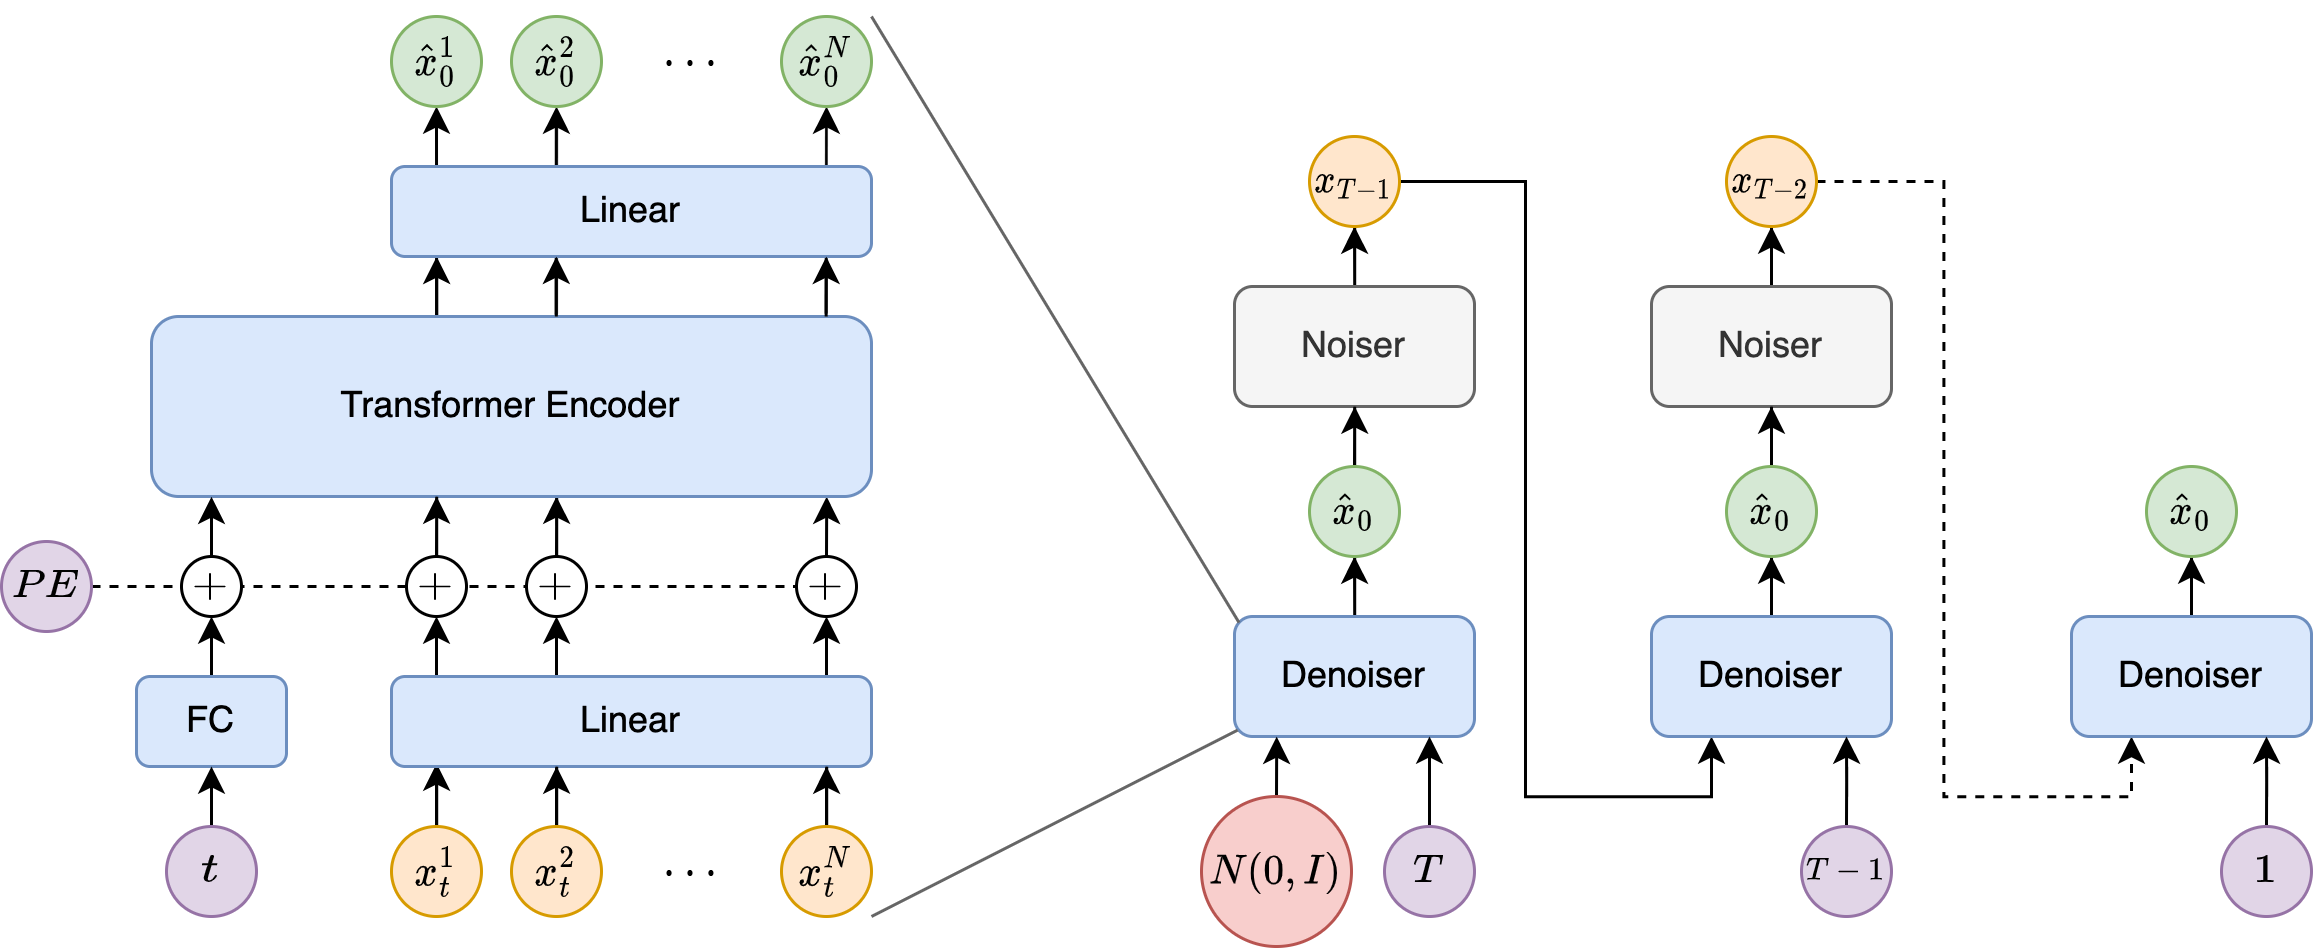
\includegraphics[width=1\textwidth]{Figures/diffusion/Network_diagram.png}
    \caption{Motion Generation - Baseline model}
    \label{fig:baseline_generation}
\end{figure}

\subsubsection{Denoising}
\TODO{Come up with a better test for this}

\subsubsection{Occluded Legs}
The model shows a strong performance on the task of inpainting missing legs in a motion sequence, with the result being of leg motion that is often both smooth and well adhering to the upper body motion. A few examples frames are shown in \figref{fig:baseline_occluded_legs}. 
The most notable failure case is that sometimes the model reverses the direction of motion. We postulate that this is due to the fact that the data for the baseline model has a root that does not move in the forward/reverse direction, therefore the pendulating rotation motion of the hips, without the additional context of a specific direction, can often be both interpreted as both forward and backward motion.

\begin{figure}[!ht]
    \centering
    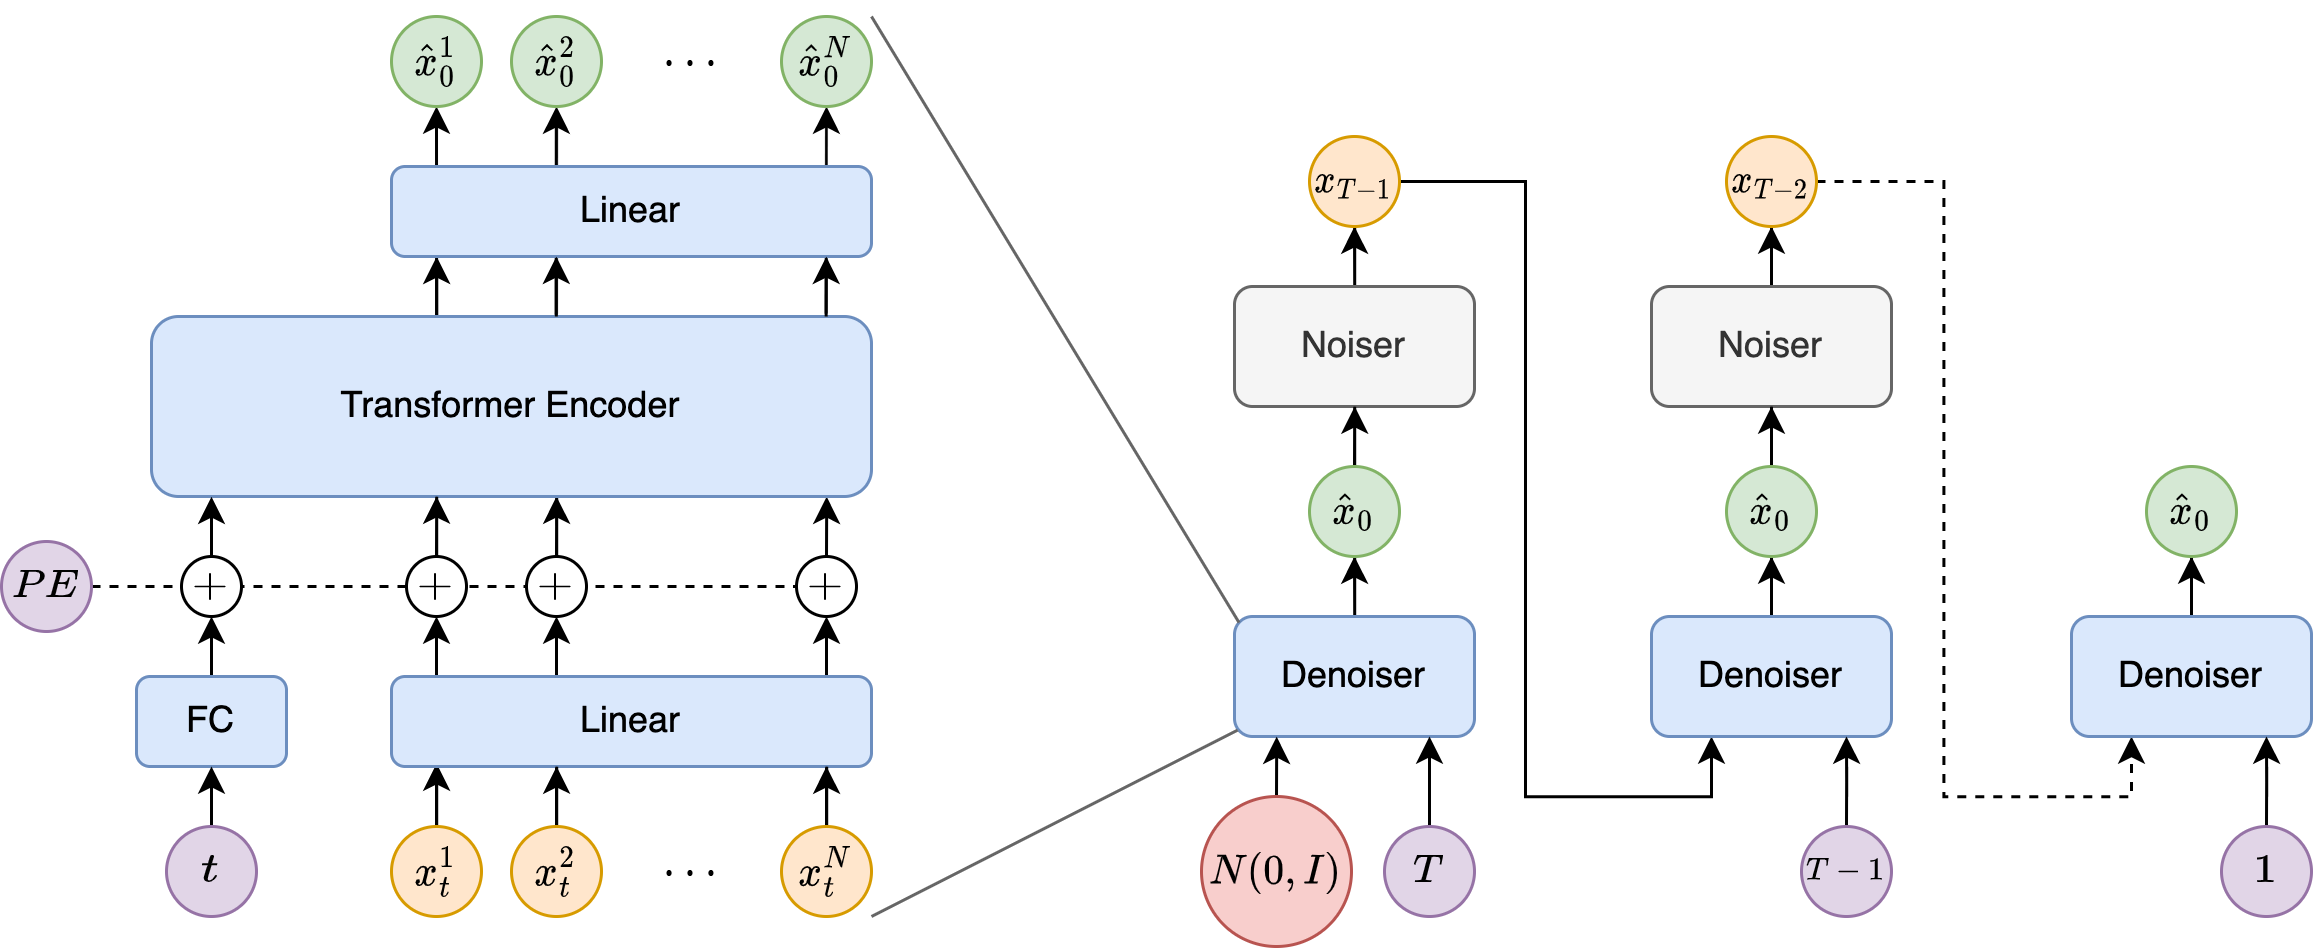
\includegraphics[width=1\textwidth]{Figures/diffusion/Network_diagram.png}
    \caption{Occluded Legs Inpainting - Baseline model}
    \label{fig:baseline_occluded_legs}
\end{figure}


\subsubsection{Missing State}
\textbf{Random each frame}
When removing a new random subset of the joints of each pose every frame in the motion sequence, we find that the model can very accurately reconstruct the missing state, even when only 50\% of the state is given each frame, and surprisingly it still performs reasonably well when only 25\% of the state is given each frame. A few example frames are shown in \figref{fig:baseline_missing_state_random_frame}. This shows that the model has learned well the concept of temporal consistency, as in this experiment it is likely that a missing joint will be surrounded (temporally) by given joints, hence it simply needs to interpolate between the given joints.

\begin{figure}[!ht]
    \centering
    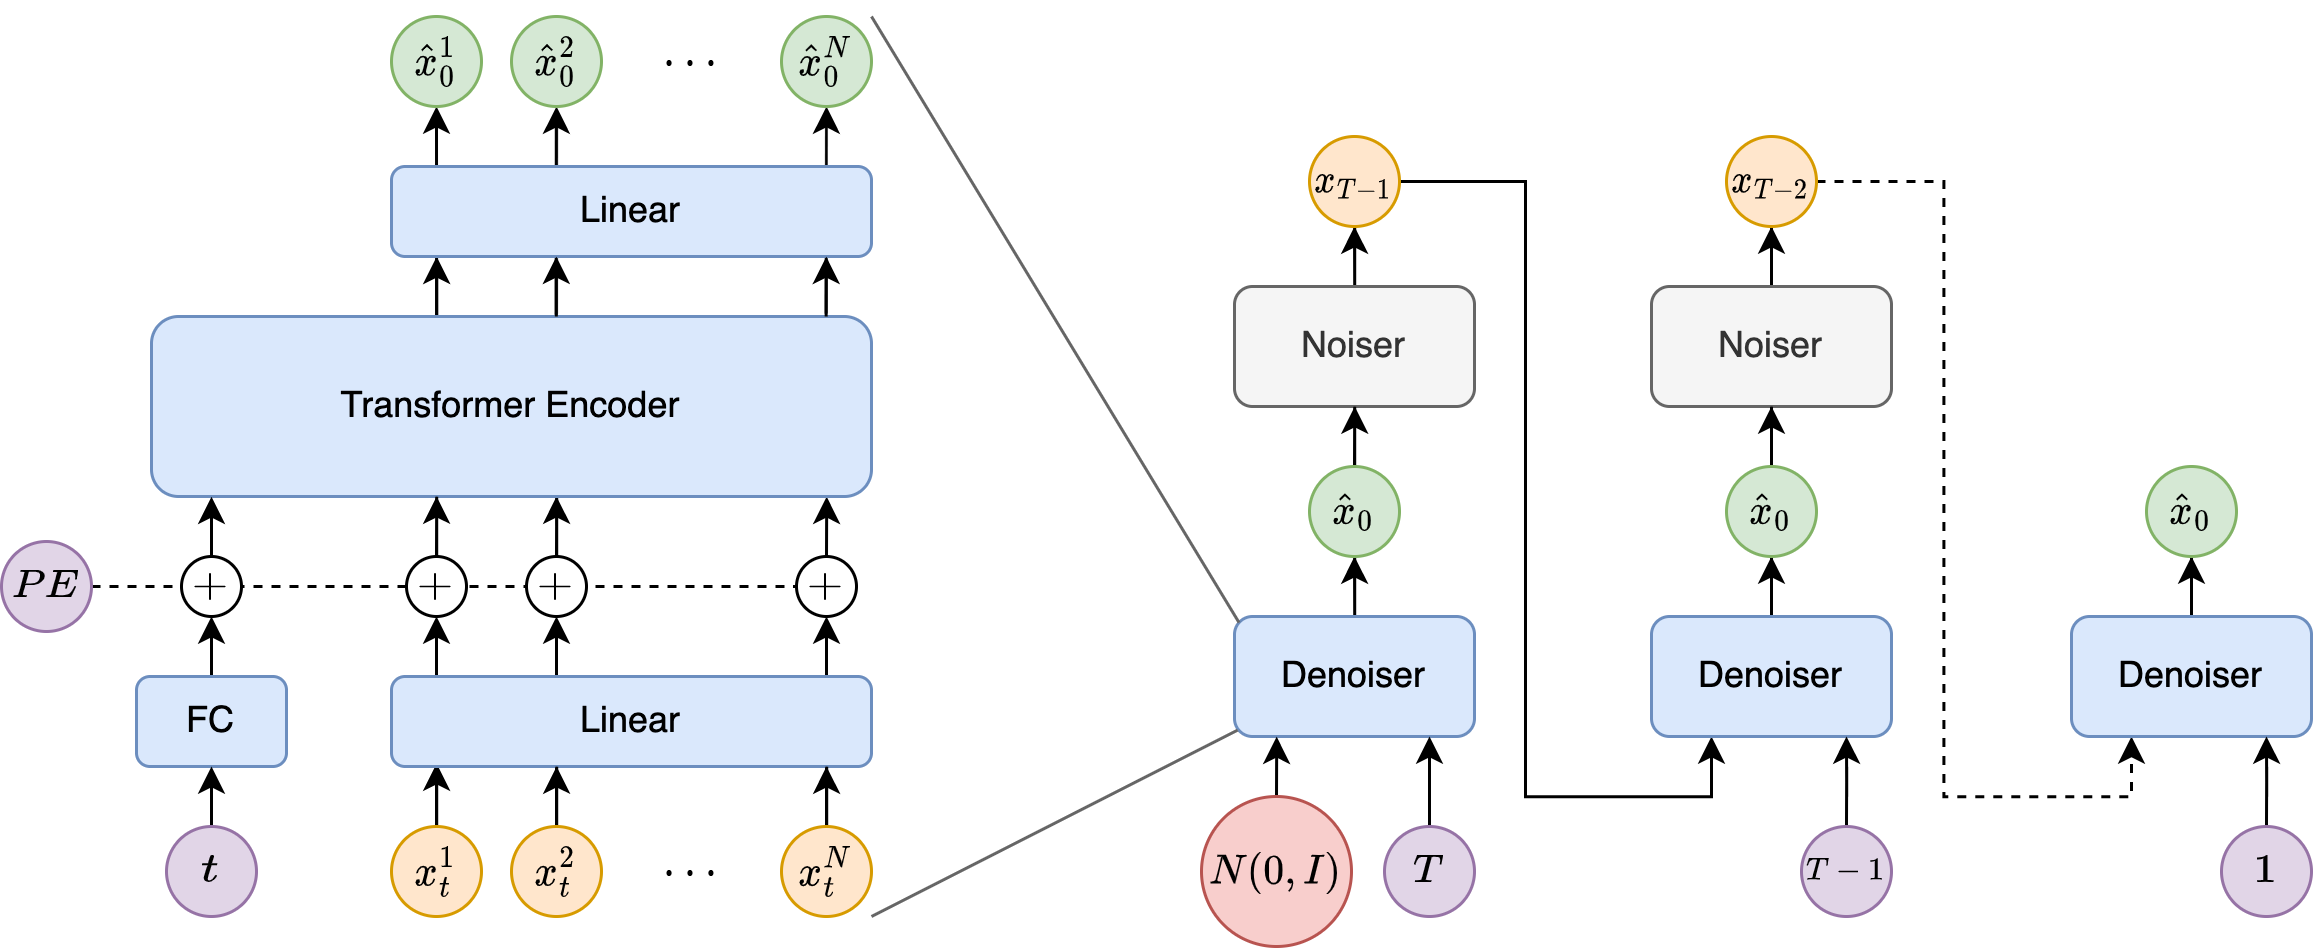
\includegraphics[width=1\textwidth]{Figures/diffusion/Network_diagram.png}
    \caption{Occluded Legs Inpainting - Baseline model}
    \label{fig:baseline_occluded_legs}
\end{figure}

\textbf{Random for the whole sequence}
\TODO{Describe better}


\subsubsection{Inbetweening}


%%%%%%%%%%%%%%%%%%%%%%%%%%%%%%%%%%%%%%%%%%%%%%%%%%%%%%%%%%%%%%%%%%%%%%%%%
% Mode with foot contacts
%%%%%%%%%%%%%%%%%%%%%%%%%%%%%%%%%%%%%%%%%%%%%%%%%%%%%%%%%%%%%%%%%%%%%%%%%
\subsection{Model with Foot Contacts}

\subsubsection{Sequence Generation}
\subsubsection{Denoising}
\subsubsection{Occluded Legs}
\subsubsection{Missing State}
\subsubsection{Inbetweening}


%%%%%%%%%%%%%%%%%%%%%%%%%%%%%%%%%%%%%%%%%%%%%%%%%%%%%%%%%%%%%%%%%%%%%%%%%
% Mode with foot contacts
%%%%%%%%%%%%%%%%%%%%%%%%%%%%%%%%%%%%%%%%%%%%%%%%%%%%%%%%%%%%%%%%%%%%%%%%%
\subsection{Autocompletion}

Another project that is running at Disney Research|Studios is that of pose autocompletion. This is the task of taking a set of \textit{handles}, a subset of joints, and predicting the position of the rest of the joints. The goal here is to again help to improve the animation pipeline, by reducing the amount of work an animator has to do to get a sensible pose. As a side note to the previous experiments, we train
ed some diffusion models for the described task, where we enforce a sequence length of 1 so that we are only predicting  single pose, and where we modify the inpainting to allow for a specific set of joints to be deemed \textit{handles} and to be kept fixed.

\subsubsection{Baseline}
The model is as described in \secref{sec:baseline_evaluation} however with a sequence length of 1.

We find that while the model does present plausible poses, and that on average these poses have handle joints close to the desired positions of the handles (with a few exceptions), it does not satisfy the task properly as can be seen in \TODO{include images of position of handles vs. position of actual joints}. An ideal solution would not move the handles at all, and would simply modify the rest of the joints.

\TODO{include images}


\subsubsection{Handle Conditioning}
To mitigate this issue of the handles being modified, we propose a handles conditioning, in which a one hot embedding of the handles is run through a linear layer, then concatenated to the input of the network. A loss is then applied to the output that penalises any deviation in position of the handles that are output as compared to those input. In theory this should force the network to learn to consider the handles as immutable, and to create a pose that satisfies the handles.

Though the implementation was largely completed, we unfortunately did not have time to finish debugging some of the finer details, and so cannot provide concrete results. However we deemed the idea interesting enough to present in this thesis, and hope that it can be of use in future research directions.